%!TEX root = ../thesis.tex
%*******************************************************************************
%*********************************** Fifth Chapter *****************************
%*******************************************************************************

\chapter{Experimental Procedure}  %Title of the Fifth Chapter
\label{chapter procedure}

\ifpdf
    \graphicspath{{Chapter5/Figs/Raster/}{Chapter5/Figs/PDF/}{Chapter5/Figs/}}
\else
    \graphicspath{{Chapter5/Figs/Vector/}{Chapter5/Figs/}}
\fi

This chapter describes the protocol of the experimental procedure along with the calculations performed in order to quantify the measurements obtained during the test. This experimental procedure and protocol gained the approval of the City University London Research Ethics Committee. Examination authorised under reference \textit{''SREC 15-16 01 E 29 09 201''} of the \nth{11} of November 2015. 

This study entailed the participation of eight healthy volunteers; six of these participants were males the remaining ones were females aged between \numrange{23}{37} years-old (mean 28.77). In accordance to the regulation of the committee, only healthy participants were allowed to take part of the research. Any participant with cardiovascular disease history did not participate in this study. 

Prior to their recruitment, the participants received the documentation which explained the entire procedure to them. Upon their approval, the party returned the consent form signed in order to schedule the study. The experiments took place at the Research Centre for Biomedical Engineering of City, University of London. Upon arrival, the participants acclimatised for \SI{10}{\min} wherein the room temperature was \SI{22(2)}{\degreeCelsius}. During this period, the experimental procedure was clearly explained to the attendant. Subsequently, the following steps were followed.

\section{Experimental procedure} %Section - 5.1
\label{section procedure 1}

After filling paperwork and completing the acclimatisation process, different instruments were used to acquire physiological signals. These measurements included ECG, PPG, laser Doppler flowmeter, Doppler ultrasound, and impedance plethysmography. Table \ref{table:instruments} describes the purpose of each instrument in this experiment. 

\begin{table}
	\caption{Instruments used during the study and measurement taken}
	\centering
	\label{table:instruments}
	\begin{tabular}{cp{0.2\textwidth}p{0.5\textwidth}}
		\toprule
		\textbf{Instrument} & \centering{\textbf{Method}} & \centering{\textbf{Measurement}} \tabularnewline \midrule
		ECG & Sense of electrical charges in heart & Electrocardiogram \tabularnewline \midrule
		PPG & Optical & Measurement of changes of volume in vascular bed \tabularnewline \midrule
		LDF & Optical & Measurement flow in capillary bed (Cell level) \tabularnewline \midrule
		iPG& Electrical & Measurement of changes of volume in a segment \tabularnewline \midrule
		Doppler Ultrasound & Electromagnetic & Measurement of flow speed \tabularnewline \midrule
	\end{tabular}  
\end{table}

The ECG device used to take the electrocardiograph was a Cardioline\textsuperscript{\textregistered} Delta 60 plus \cite{remco:delta60} using a 4 electrodes configuration. The Zen PPG registered the photo-plethysmographic waveform using a finger sensor that operated with a light source at \SI{680}{\nano\meter}. The LDF instrument used in the course of this experiment was the moor VMS-LDF2 \cite{moor:LDF2}. This instrument worksusing a laser light at a wavelength of \SI{785}{\nano\meter}. The Doppler ultrasound was a Huntleigh Healthcare MD2 instrument with a sensor head of \SI{8}{\mega\hertz} \cite{ht:MD2}. Finally, the iPG device that was described in the previous section was used to take the impedimetric readings. 

\subsection{Instruments set-up}
\label{section procedure 1.1}

Before attaching any instruments to the participants, physical dimensions needed to be taken from them. This data was needed to be convert some of the physiological measurements to meaningful numbers. For instance, the quantification of impedance plethysmography requires the knowledge of the geometric shape of the volume being measured. Hence, it necessitated a recording of the forearm's segment volume by weighing both length and circumference. Additionally, the distance from heart to shoulder, upper arm length, and shoulder to index finger length was also recorded as reference points. 

Next, all the participants sat in a comfortable chair. Their left arm rested on a soft cushion atop a table placed next to a chair that was adjusted to collaborator's height. Subsequently, blood pressure was taken using an automated instrument by recording diastolic and systolic values for each one. Subsequently, each participant positioned ECG electrodes on themselves to form an Einthoven triangle. According to the device's instructions, electrodes need to be placed on each shoulder and ankle. Leads were secured to the electrodes in order to verify that ECG signal was clean. The apparatus includes an output port that exports the waveform for further processing. 

As the next step, a PPG probe was placed on the index finger. The PPG instrument is a device designed by the biomedical research group of City University, known as Zen PPG. This equipment has two available channels, but the experiment required just one port. Each channel provides two outputs containing AC and DC components of the photoplethysmographic waveform. 

Next, the laser Doppler Flowmetry probe~\cite{moor:LDF2} was attached on the forearm's mid-section. This device detects moving red blood cells within a vessel below the vascular bed in the skin. In addition, this device has an external analogue port where the acquired signal can be exported for post-processing.  

The Ultrasound Doppler probe was then placed as close as possible to the radial artery. When the probe is placed closed to the main vessel, the speed of blood flow produces a unique audible signal. However, calculating blood flow from this signal requires a set of distinct skills by placing the probe at a fixed angle and maintaining closeness to the artery for a good measurement. Therefore, the probe head of the instrument needs to be placed at a fixed angle. Hence, the instrument's head was secured using a laboratory stand and clamp that was pointing at the party's radial artery on the wrist. The appliance also features an external port for additional processing.  

Finally, the impedance plethysmography electrodes were placed on the forearm's skin. To do so, ECG electrodes were used since they provide a good contact point, which is essential to carry out the experiment successfully. The current probes were placed following the path of the left radial artery; one below the elbow (brachial artery) and the second one on top of the radial artery close to the wrist. Potential electrodes were situated next to the previous electrodes towards the underneath portion of the forearm. The diameter of the circumference around these electrodes was recordedalong with its distance separation. These physical measurements facilitate the calculation of the volume of the forearm's segment that isto be measured. The total volume of that portion of the arm was calculated using the equation \ref{eq:v_e}.

\begin{align}
	\label{eq:v_e}
	V_e =\frac{l \times (C_1^2+C_1 \times C_2 + C_2^2)}{(12 \times \pi)} \tagaddtext{[\si{\cubic\centi\meter}]}
\end{align}

where $V_e$ denotes the segment's volume, $l$ represents the length between the potential electrodes, and $C_1$ and $C_2$ are the circumference measurement at elbow and wrist electrodes, respectively.

The entire experiment set-up is illustrated in figure \ref{fig:experimental set-up} where all the instruments and its positions are recorded.

\begin{figure}[!htpb]
	\centering
	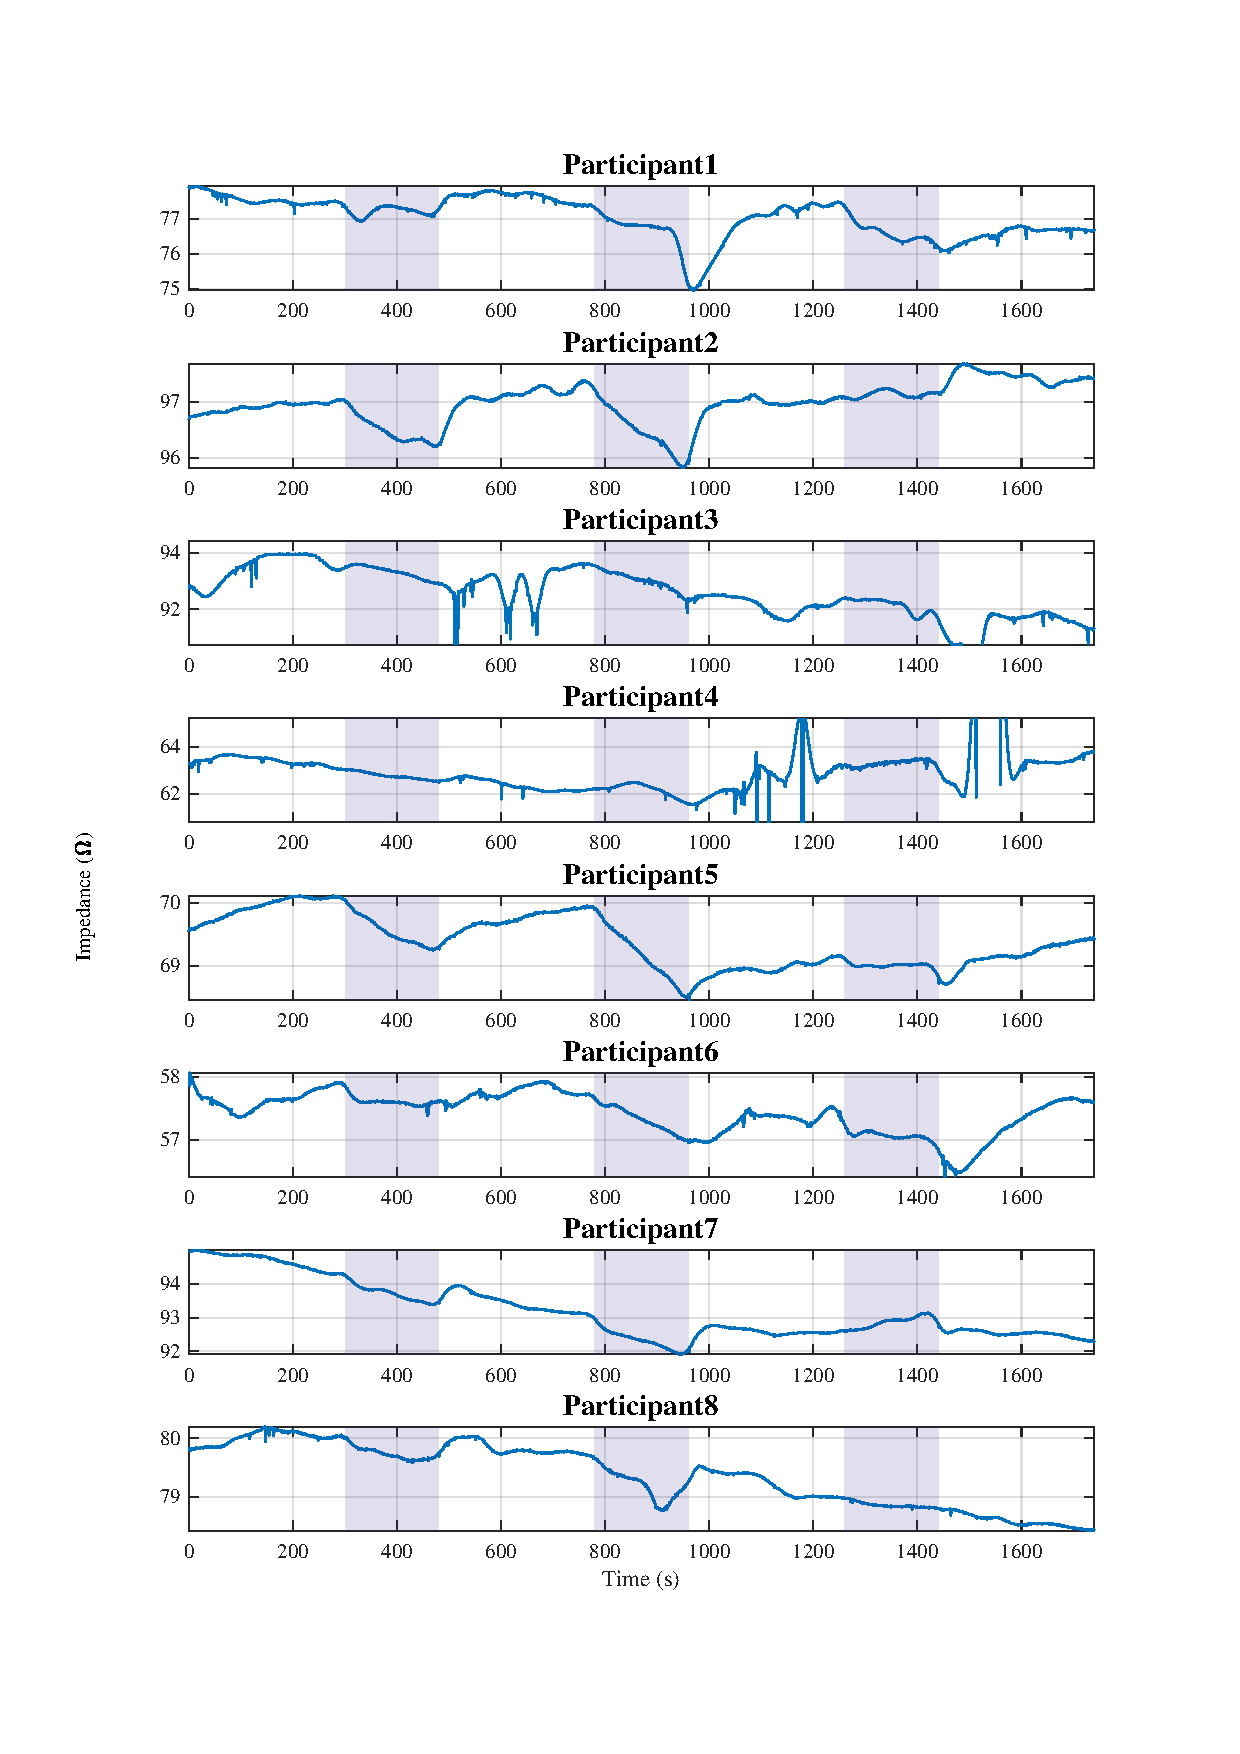
\includegraphics[width=15cm,keepaspectratio]{figure1}
	\caption{Position of all the instruments during the experiment in the forearm}
	\label{fig:experimental set-up}
\end{figure}

\subsection{Physiological measurements}
\label{section procedure 1.2}
As noted before, physiological measurements of the participants were takenat the beginning of the study to collect data like age, sex and arm to heart distance. The table \ref{tbl:physiological} summarises the information provided by all the participants. The ages of participants ranged between \SIrange{23}{37}{year-old} (mean \num{29.12(494)}). 

\begin{table}[!ht] %tbl:physiologica
	\caption{Participants' age, sex and forearm measurements}
	\label{tbl:physiological}
	\centering
	\begin{tabular}{lcc|ccc}
		\toprule
		&&&         \multicolumn{3}{c}{\textbf{Dimensions [\si{\cm}]}}         \\
		& \textbf{Age} & \textbf{Sex} & \textbf{Arm length} & \textbf{Shoulder} & \textbf{Total length} \\
		&&&&  \textbf{to heart}   &                       \\ \midrule
		Participant 1 &      26      &     Male     &         80          &          26          &          106          \\
		Participant 2 &      23      &    Female    &         66          &          24          &          90           \\
		Participant 3 &      27      &    Female    &         74          &          24          &          98           \\
		Participant 4 &      37      &     Male     &         68          &          24          &          92           \\
		Participant 5 &      29      &    Female    &         62          &          24          &          86           \\
		Participant 6 &      36      &     Male     &         70          &          24          &          94           \\
		Participant 7 &      29      &     Male     &         73          &          23          &          96           \\
		Participant 8 &      26      &     Male     &         69          &          23          &          92           \\ \bottomrule
	\end{tabular}
\end{table}

In addition to these measurements, the distance between impedance potential electrodes and the arm circumference was simultaneously recorded using a measuring tape. This data makes it possible to estimate the forearm's segment total volume by gauging the total distance between the potential electrodes ($l$), and the circumference of each electrode's location (C$_1$ and C$_2$). Table \ref{tbl:measurments} illustrates the dimensions of the participant's forearm between the sensing electrodes and the segment's volume as calculated from Equation \ref{eq:v_e}.

Using a measuring tape to accommodate these dimensions may induce some errors in the data. For instance, applying excessive pressure on the arm, when taking the measurements, may provide a lower circumference value. However, this also allows estimating the initial volume of the forearm segment which signifies the original volume of the conductive portion. 

\begin{table}[!htbp] %tbl:measurments
	\caption{Participants' forearm dimensions and initial total volume}
	\label{tbl:measurments}
	\sisetup{separate-uncertainty=true}
	\centering
	\begin{tabular}{lcccccc    S[table-format=2.2]@{\,\( \pm \)\,}S[table-format=1.2]}
		\toprule
		&  \textbf{L [\si{\cm}]}   &  \textbf{C$_1$ [\si{\cm}]}  &  \textbf{C$_2$ [\si{\cm}]}  &   \textbf{Ve [\si{\cubic\cm}]} \\\midrule
		Participant 1 & 14.8 & 17.5 & 27.5 & 606.05 \\
		Participant 2 & 11.0 & 15.0 & 20.0 & 269.90 \\
		Participant 3 & 13.0 & 19.0 & 26.5 & 540.27 \\
		Participant 4 & 10.0 & 17.5 & 25.0 & 363.07 \\
		Participant 5 & 10.0 & 17.5 & 23.5 & 336.81 \\
		Participant 6 & 11.0 & 18.5 & 27.0 & 458.32 \\
		Participant 7 & 13.5 & 15.0 & 23.0 & 393.55 \\
		Participant 8 & 11.5 & 17.0 & 23.5 & 378.49 \\ \bottomrule
	\end{tabular}
\end{table}

\subsection{Experimental protocol}
\label{section procedure protocol}

One of the key endeavours of this experiment is to look into iPG waveform alterations in case of an obstruction in the blood flow towards the forearm. It is possible to restrict  blood circulation in this area by applying a mechanical blockage on the upper arm using a standard inflatable blood pressure instrument. The device necessitates being pumped manually using an inflation bulb. A gauge in the instrument is indicative of the cuff pressure level. This cuff was secured on the left biceps of the participant. 

The protocol entailed the recording of three different types of blood flow occlusion. The first kind restricts blood flow return by blocking the venous circulation through a technique known as Venous Occlusion Plethysmography (VOP). This method is extensively used to assess peripheral circulatory problems  described by Wilkinson et al. \cite{wilkinson2001venous}. This obstruction can be produced by inflating the cuff usually just below the diastolic pressure between \SIrange{10}{20}{\mmHg}. Therefore, blocking the upper arm obstructs blood flow within the median cubital and basilic veins without obstructing the brachial artery's arterial inflow.  Overall, the target pressure was \SI{20}{\mmHg} for each participant under their diastolic pressure recorded at the start of the session.

A partial arterial occlusion (PAO)was the second class of blood flow limitation. This kind of blockage lowers the amount of arterial blood coming into the forearm, but also impedes venous blood return. Studies have demonstrated that constricting an artery lowers the arterial flow towards the periphery \cite{uchida1977cyclical}. For instance, this can be obtained by applying a mechanical compression on the upper arm between diastolic and systolic pressures, thereby intensifying the wall pressure of the brachial artery. Therefore, the prime objective was to constrict the upper arm as regards to the mean value between diastolic and systolic pressure. For that purpose, the calculation was made using the following equation.

\begin{align}
	\label{eq:meanpressure}
	P_m = \frac{P_d + P_s}{2} \tagaddtext{[\si{\mmHg}]}
\end{align}

where $P_d$ is diastolic pressure and $P_s$ is systolic pressure. 

The last kind of occlusion needed is total occlusion (TO), which makes it possible to occlude above systolic pressure. Also known as "Suprasystolic" or "stop-flow", it can provide valuable tonometric information \cite{lowe2009non}. In this experiment, blood flow was blocked by inflating the cuff higher than \SI{20}{\mmHg} of participant's systolic value that was previously measured. This method of occlusion completely restricts the inflow and outflow of venous and arterial blood. Hence, no change of volume is expected to take all along this part of the test.

\subsubsection{Blood pressure occlusion estimation}
Obtaining blood pressure levels requires a record of blood pressure for each participant. Therefore, before commencing the study, three readings of blood pressure were taken and averaged per participant using an automated blood pressure instrument brand Omron IntelliSense (Omron Healthcare). The mean systolic and diastolic pressures of all the partakers of this investigation were \SI{116.25(1366)}{\mmHg} and \SI{72.75(723)}{\mmHg} respectively. The venous occlusion level was targeted at \SI{20}{\mmHg} below systolic pressure the total mean was \SI{55.00(801)}{\mmHg}, the partial arterial pressure was calculated using the equation \ref{eq:meanpressure}, the average was about \SI{94.63(1021)}{\mmHg} and total occlusion was around \SI{136.25(1367)}{\mmHg}. Table \ref{tbl: venous occlusions} details the blood pressures recorded per participant.

\begin{table}[!htbp] %tbl: venous occlusions
	\caption[Blood pressure and occlusion levels of the participants]{Participants' initial blood pressure and levels for venous, partial arterial and total occlusion}
	\label{tbl: venous occlusions}
	\centering
	\begin{tabular}    {lcccc}
		\toprule
		& \textbf{Blood pressure}  &  \textbf{Occlusion 1}   & \textbf{Occlusion 2}  &  \textbf{Occlusion 3} \\
		&  [\si{\mmHg}]   &        [\si{\mmHg}]  &    [\si{\mmHg}]   &  [\si{\mmHg}]\\ \midrule
		Participant 1  &  124/78   &        50  &    101   &  144\\ 
		Participant 2  &  105/65   &        50  &     85   &  125 \\
		Participant 3  &  120/78   &        60  &     99   &  140 \\
		Participant 4  &  120/72   &        60  &     96   &  140 \\
		Participant 5  &  100/60   &        40  &     80   &  120 \\
		Participant 6  &  143/82   &        60  &    113   &  163 \\
		Participant 7  &  107/73   &        65  &     90   &  127 \\
		Participant 8  &  111/74   &        55  &     93   &  131 \\\bottomrule
	\end{tabular}
\end{table}

Based on the data from table \ref{tbl: venous occlusions} it was possible to set the parameters for this experimental procedure. The column \textit{occlusion 1} establishes the proper pressure for venous occlusion plethysmography (VOP). With the pressures coming in from column \textit{occlusion 2} the arterial blood flow was restricted along with the venous return. Finally, \textit{occlusion 3} presents information about the changes of impedance during total occlusion.

\subsection{Data acquisition}
\label{section procedure 1.4}

All instruments used in this experiment provided the external ports for further data processing. These output ports were connected to a DAQ NI-6211 (National Instruments). This analogue to digital converter card provides as many as 32 channels along with a combined sampling rate of \SI{250}{\kilo\sample\per\second}. The DAQ is connected to a personal computer using USB port (Version 1.0). All signals were sampled at \SI{1}{\kilo\hertz} with a reference voltage between \SIrange{0}{10}{\volt} for the iPG channel $Z_{DC}$ and \SI{\pm 5}{\volt} for the other signals. Therefore, the resolution of DAQ was \SI{152.6}{\micro\volt}, which was calculated using equation \ref{eq:resolution}. 

\begin{align}
	\label{eq:resolution}
	Res =\frac{V_{p-p}}{2^{n}}		\tagaddtext{[\si{\volt}]}
\end{align}

where $V_{p-p}$ denotes the reference voltage peak to peak with $n$ being number of bits used to sample the signal. 

A virtual instrument using LabView \cite{LabView:2016} was created to display, process and store raw data. Figure \ref{fig:experimental set-up 2} shows the front-end of the program. The programmed custom virtual instrument shows four distinct channels of waveforms. For the purpose of this experiment iPG, ECG, PPG and Ultrasound Doppler were among those that were selected for portraying the signals.

\begin{figure}[!htpb]
	\centering
	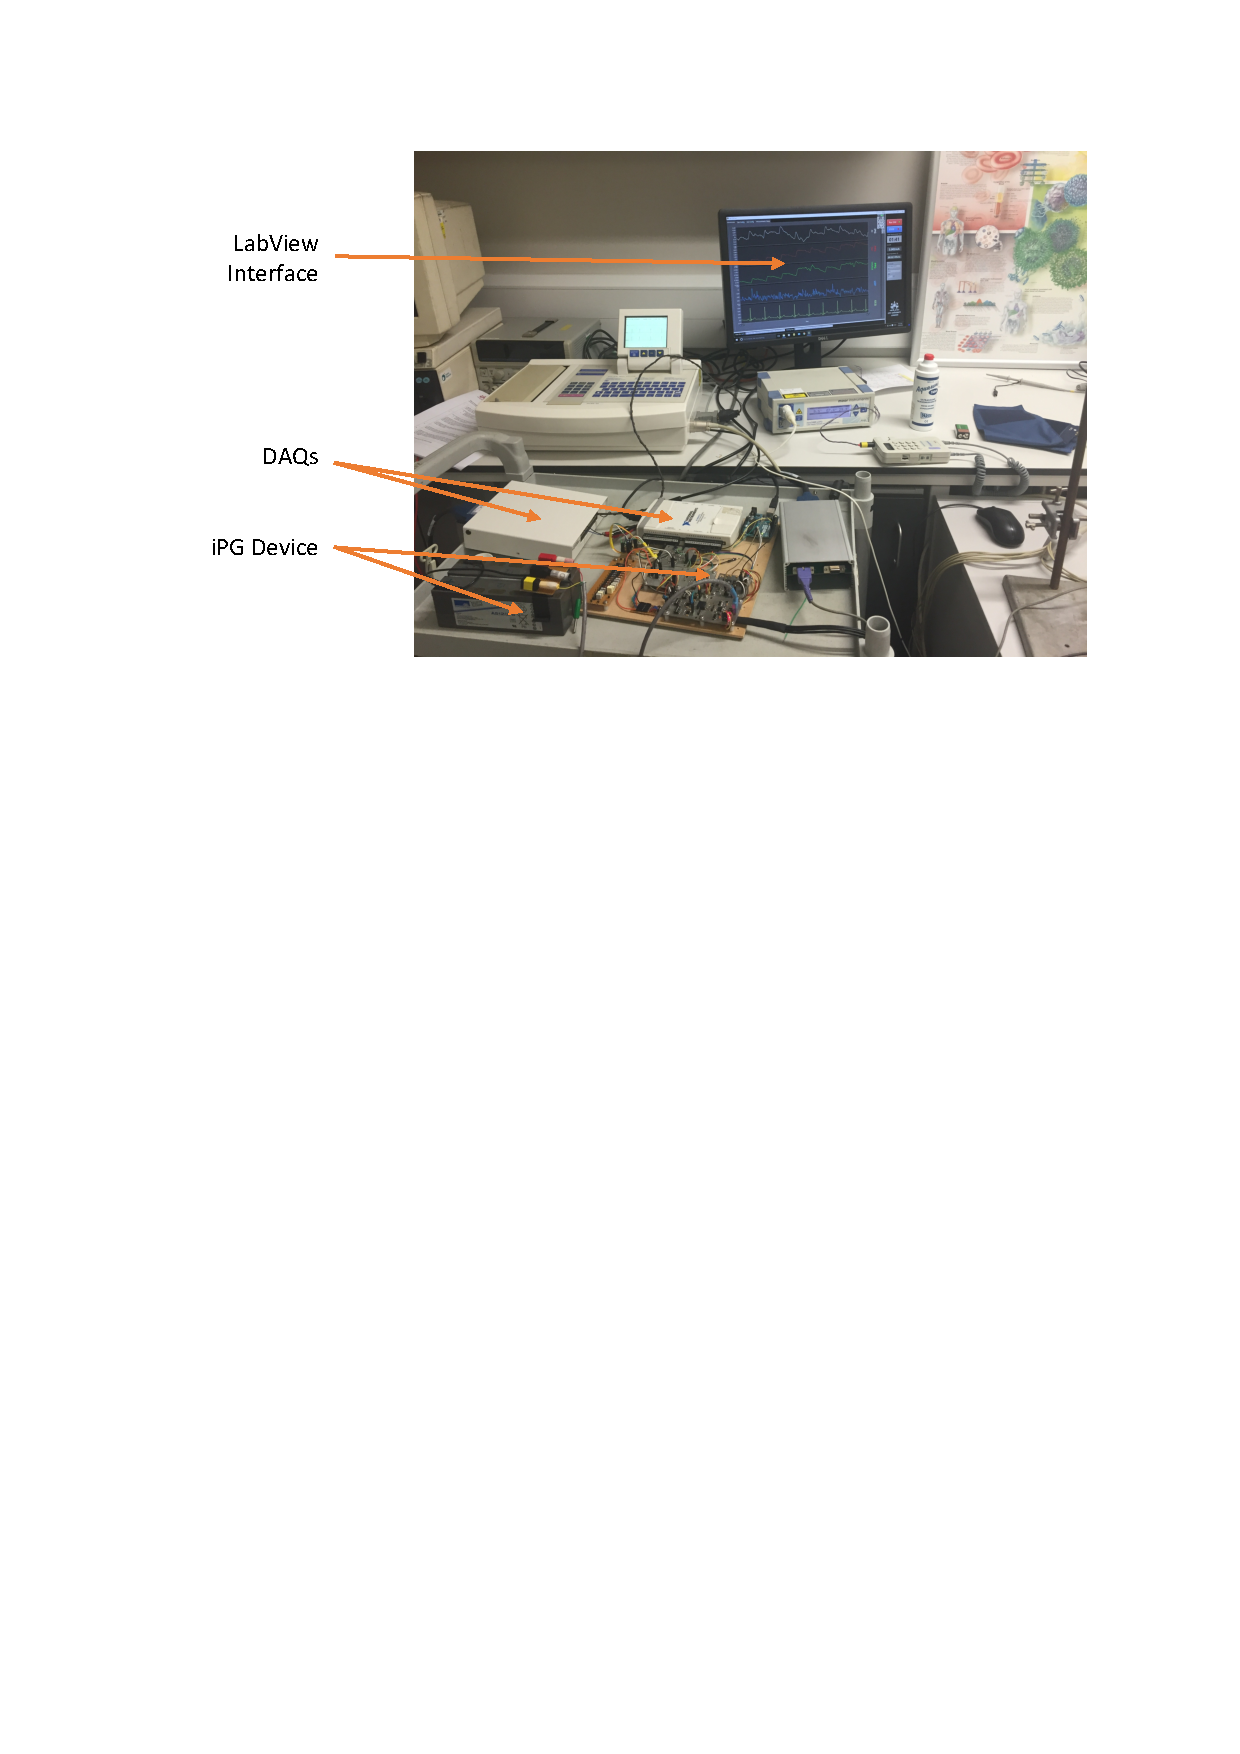
\includegraphics[width=15cm,keepaspectratio]{figure2}
	\caption{Additional instruments used during the experimental procedure}
	\label{fig:experimental set-up 2}
\end{figure}

For displaying purposes, band-pass filters were applied to the iPG and PPG signals, removing unwanted DC components as well as high frequency noises. The waveforms from other instruments did not necessitate filtering since the devices served clean signals. 

The virtual instrument also included configuration capabilities. Two tabs in the program featured a field for physical measurements, general application settings and other adjustment for the PPG instrument. The participant tab required the following: left arm dimensions, blood pressure and file path name. Meanwhile in the second tab, the VI adjusts the light intensity of this PPG probe. Generally, a \SI{20}{\milli\ampere} is sufficient to provide a good amplitude signal. At the end of this experimental procedure, all raw data was stored on an LVM file created by LabView.

The main panel apart from the one that just displayed waveforms includes control buttons and a timer.  Pressing the start button commences a timer and stores data waveform in the memory. Pushing the same button again stops the timer and saves the entire data in a local LVM file. 


\subsubsection{Recording waveforms}
At this point, after recording all physiological measurements operating all instruments successfully, a small test was carried out. Even as the waveforms were being shown on the screen, \SI{2}{\min} of recordings were taken, although it was not recorded. Participants were advised to limit their movements during this experiment. 

As soon as all signals were readable and noise free, the start button of the VI was pushed to initiate the study. At the commencement, \SI{5}{\min} of baseline recordings were obtained. These waveforms provided the standard control wave that could be compared with occluded waveforms. Then, immediately after the timer reached this time, the cuff was inflated rapidly to \SI{20}{\mmHg} below the diastolic pressure, thus producing venous occlusion along with an increment in the total volume of the forearm of blood pooling effect. This level of blockage was held for \SI{3}{\min} followed by swiftly deflating the cuff. 

The next step required producing the partial arterial occlusion using similar time spans as the ones that were used during venous occlusion. As described previously in the literature, reperfusion following an occlusion does not affect blood pressure, heart rate or blood flow \cite{kharbanda2002transient}. Hence, \SI{5}{\min} provides sufficient time to restore the blood flow to normal limits. It is for this reason that the cuff's air valve was left open to bleed all the air inside. Subsequently, the cuff was quickly inflated again until the pressure calculate in equation \ref{eq:meanpressure} was reached. The cuff's pressure was maintained at this level for \SI{3}{\min} followed by a quick release of pressure.

Last, a similar method was appliedfor total blood occlusion. Yet again, \SI{5}{\min} of baseline waveforms were taken followed by a fleeting cuff inflation to \SI{20}{\mmHg} above the diastolic pressure. This compression was kept for \SI{3}{\min}. At this point, maintaining this tourniquet effect can become painful after a couple of minutes. As a result, some of the helpers ended up re-accommodating motion artefacts in the data. 

Finally, the last \SI{5}{\min} of baseline waveforms were recorded in order to study the recovering effect. When the time was up, the stop button was pushed to save the entire data onto an LVM file for further processing in Matlab \cite{MATLAB:2016}. Figure \ref{fig:pressure applied} illustrates the pressure levels applied during the entire experiment.

For a better understanding of the different stages of this experiment, each event was identified as a region. Thus, the regions 1, 3, 5 and 7 represent the non-occlusive events or baseline readings. In contrast, regions 2, 4 and 6 are equivalent to VOP, PAO and TO events.

\begin{figure}[!htpb]
	\centering
	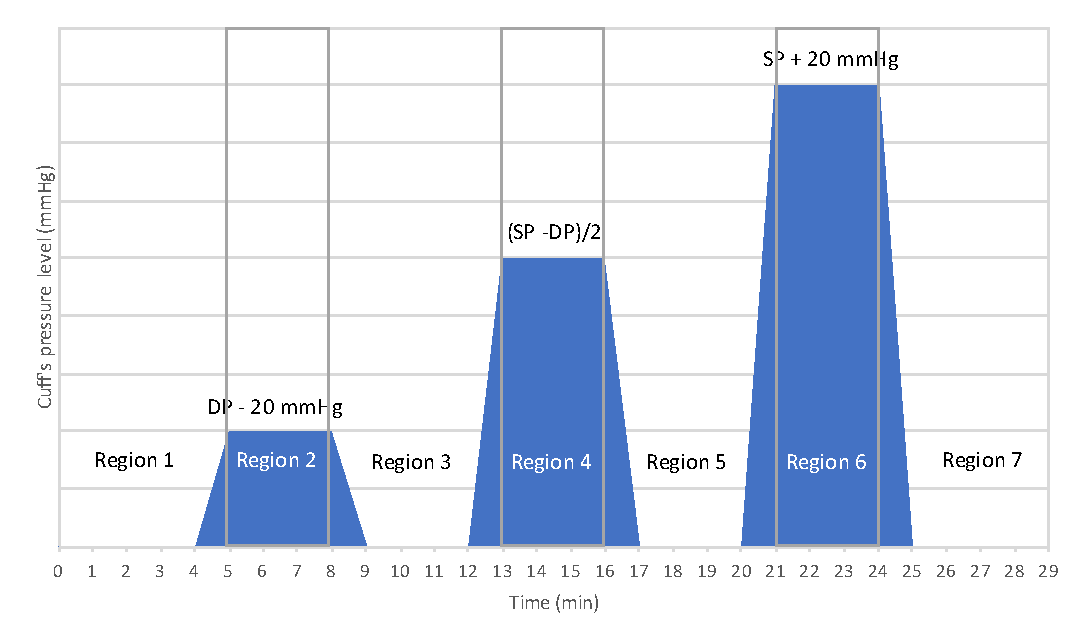
\includegraphics[width=15cm,keepaspectratio]{figure3}
	\caption[Pressure and rdescription of regions during the experiment]{Pressure applied to the participant during the experiment. The clear areas represent the resting period of \SI{5}{\minute}, and the shaded areas denote the pressure applied at the desired level during \SI{3}{\minute}. All the regions have been denoted for reference during the analysis}
	\label{fig:pressure applied}
\end{figure}

\section{Data processing}
\label{section procedure 2}
Once the data was collected and saved in the LVM format, the waveforms were post-processed in Matlab \cite{MATLAB:2016}. A Graphic User Interface (GUI) Matlab program was created to compare four waveforms time while simultaneously applying filters, finding peaks and windowing different sections of data. A front-end of the application can be seen in figure \ref{fig:Matlalb Interface}.

Importing the LVM file into Matlab merely requires the extraction of the most relevant information. Therefore, a parsing program was created where unwanted headers and columns of unnecessary data were removed. One of the major challenges in the data importing process was the size of LVM file. While the sampling at \SI{1}{\kilo\hertz} provided great detail of the waveforms, it also created files of approximately \SI{300}{MB}. Importing this file size drastically slowed down the workstation. Therefore, data was decimated in a magnitude of ten while being imported into Matlab. Consequently, each physiological waveform was reduced to less than \SI{1}{MB} of size whilst maintaining a good waveform detail. 

Notably, this data decimation does not impact the waveform data. In fact, according to Nyquist rate, data was oversampled. Physiological signals are between \SIrange{1}{2}{\hertz} depending on the heart rate. According to the Nyquist theorem, up to \SI{4}{\hertz} would have provided sufficient sampling frequency for the waveforms \cite{nyquist1928certain}. Nevertheless, a sampling of \SI{100}{\hertz} is enough to accommodate a high resolution of the discrete-time signal. Even so, including oversampled signals was not random. It allows the implementation of high order digital filters with sharp cut-off frequencies. 

\begin{figure}[!htpb]
	\centering
	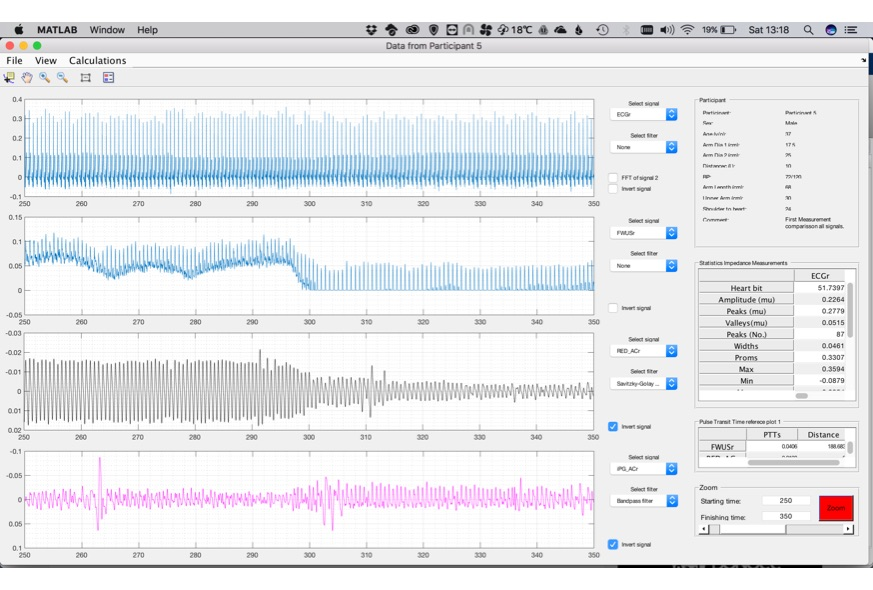
\includegraphics[width=15cm,keepaspectratio]{figure4}
	\caption[Graphic user interface of the Matlab application]{Graphic user interface of the Matlab application used to qualify data and post-processing the signals acquired}
	\label{fig:Matlalb Interface}
\end{figure}

After importing decimated data into Matlab, the parsing program converted and saved each waveform into a Matlab file format (.mat). Placing the data into this kind of file accelerates the loading in memory (of the data) and the waveform presentation within the GUI. Another advantage of such a file conversion is that data processing can be performed online without using extensive computing resources. 

The end data represents volts of the physiological measurements that were captured during the experiment. It is for this reason that the information must be converted into more meaningful data. The following section describes the mathematical process to convert the signals taken from volts into equivalent measurements.

\subsection{Data conversion}
\label{section procedure data conversion}
The data imported into the GUI represents the volts of the entire physiological measurements. Therefore, this information must be converted into significant values that denote the physical variable. For instance, the signals from port $Z_{DC}$ of the iPG device is merely the potential measurement of the forearms, and not the net impedance. Converting this reading correctly into impedance necessitates the division by the current driven by the device. From this value, other physiological measurements such as volume and blood flow can also be derived. In addition, extra filtering must be applied to isolate certain characteristics of the waveforms. 

The same situation holds true for the readings taken from the Ultrasound Doppler and the Laser Doppler Flowmetry. The collected signals are only the raw data in volts which need to be converted to the right scale. The following section describes the mathematical equations and tools used to convert the raw signals effectively in greater detail.

\subsubsection{Calculation of the basal impedance value}
Impedance plethysmography signals must be converted from volts and current values into its standard scale, which is Ohms ($\Omega$). The iPG device has a channel for current sense known as $I_{DC}$, whose voltage is equivalent to the peak value of the current that is being delivered by the instrument. The effective electrical current in amperes ($A$) can be calculated by the gain relation of the various stages of the signal path. In accordance to the circuit schematic (see figure \ref{fig:mhc}), the electrical current is being sensed by a \SI{10}{\ohm} resistor $(R_s)$ in the module \textit{Modified Howland Amplifier module} (see section \ref{section MHC}). Subsequently, this signal is amplified by an instrumentation amplifier in the \textit{current and voltage sensing module} (see section \ref{section V&I sense}) which gain $(G_1)$ was fixed to \num{276}. Following the signal path, the waveform is fractioned by the super-diode circuit, which acts as a half-wave rectifier in the \textit{envelope detection module} (see section \ref{section material envelope}). The hold circuit keeps the DC voltage constant at the signal output, which is equivalent to the peak value of the current in volts. Thus, the electrical current in amperes can be calculated using the equation \ref{eq:current}.

\begin{align}
	\label{eq:current}
	I = \frac{V_{IDC} \times 2}{R_x \times G_1} = \frac{V_{IDC} \times 2}{276 \times\ 10 \Omega} = \frac{V_{IDC}}{1380 \Omega} \tagaddtext{[\si{\ampere}]}
\end{align}

The second channel of this iPG device labelled $Z_{DC}$ produces a DC voltage tantamount to the impedance of the forearm. Similarly, as the current senses voltage path, the channel passes through a series of circuits that amplifies the original potential being sourced from the forearm's segment. Therefore, the actual voltage detected by the device can be debunked by the numerous gains involved during the signal path. 

First, the unknown load is sensed by the potential electrodes ($E_2$ and $E_3$ in figure \ref{fig:electrode}) directly connected to the \textit{voltage sense module} (see section \ref{section V&I sense}). The instrumentation amplifier (AD8421) of this module was configured to a gain \num{35.65}. In the \textit{envelope detection module} (see section \ref{section material envelope}), the signal was rectified using the super-diode circuit and halving the signal amplitude. As a result, the voltage can be deducted by using equation \ref{eq:vzdc}.

\begin{align}
	\label{eq:vzdc}
	V_z = \frac{V_{ZDC} \times 2}{35.65} \tagaddtext{[\si{\volt}]}
\end{align}

where $V_{ZDC}$ denotes the DC voltage coming from the port $Z_{DC}$.

Finally, the impedance value can be computed by converting the voltage into impedance using Ohm's law \cite{ohm1827galvanische}. This can be accomplished by replacing equation \ref{eq:current} and \ref{eq:vzdc} into \ref{eq:impedance}. The GUI programmed in Matlab automatically carries out this impedance conversion when the signal gets loaded in the GUI. This mathematical operation is undertaken by a point-to-point division between the two signals after subtracting their gains from their raw values. 

\begin{align}
	\label{eq:impedance}
	Z = \frac{v}{i}=\frac{V_z}{I} \tagaddtext{[\si{\ohm}]}
\end{align}

\subsubsection{Calculation of the Arterial Pulse Amplitude value}
The third channel is the APA signal designated as $Z_{AC}$. This waveform is an amplified version of the dynamic signal within $Z_{DC}$. During the course of analysing the signal's path, it can be seen that thetwo circuits work on the waveform in tandem. First, it is the circuit from where this signal originates which is the same voltage as seen in port $Z_{DC}$, implying that the gain described in the previous section also has an impact on the signal $Z_{AC}$. The second circuit which affects the signal is the band-pass filter within the \textit{envelope detection module} (see section \ref{section material envelope}). As can be appreciated in figure \ref{fig:envelope detector voltage}, this filter entails a fixed gain of \num{142.42} and eliminates any kind of DC and high-frequency noise components. Subsequently, the voltage of the plethysmography wave can be found by combining both gains using the equation \ref{eq:ViPG}.

\begin{align}
	\label{eq:ViPG}
	V_{APA} = \frac{V_{ZAC} \times 2}{142.42 \times 35.65}=\frac{V_{ZAC}}{2538.66} \tagaddtext{[\si{\volt}]}
\end{align}

where $V_{ZAC}$ denotes the raw AC voltage coming from the port $Z_{AC}$.

Likewise, the dynamic signal's impedance value ($Z_{AC}$) can be calculated using Ohm's law \cite{ohm1827galvanische} by replacing the APA voltage from equation \ref{eq:ViPG} as well as current from equation \ref{eq:current}. In Matlab, this impedance value is calculated as soon as the signal gets selected by applying this mathematical formula.

\begin{align}
	\label{eq:zipg}
	Z_{iPG}=\frac{v}{i} = \frac{V_{APA}}{I} \tagaddtext{[\si{\ohm}]}
\end{align}

\subsubsection{Converting ultrasound to flow}
\label{sectionDU}
The instrument used in this study was a Huntleigh model MD2 with sensor type VP8. The frequency of the transmitter is \SI{8}{\mega\hertz} which makes it ideal for blood flow estimation. The principle of this device pertains to the frequency of a source to its velocity relative to a sensor \cite{surgeonhand2002Hand}. Put simply, if an electromagnetic wave gets transmitted at a fixed frequency and is reflected by a moving body, the frequency of the received signal will be shifted \cite{ht:MD2}.  

The device can detect moving blood cells inside a vessel. When a cell passes through the electromagnetic beam, a frequency shift occurs that is proportional to the blood flow velocity. Nevertheless, this Doppler shift is also affected by the angle of the head of the probe along with the direction of the flow \cite{surgeonhand2002Hand}.

Since the average velocities found in the human body lies within the hearable frequency range, the device reproduces this as an audible sound with the help of a speaker. The apparatus has an output channel that produces the equivalent analogue signal for further processing. According to the service manual of this instrument, a \SI{3.5}{\volt} signal equals to a \SI{8}{\kilo\hertz} shift signal at the output \cite{ht:MD2}. Keeping this voltage as a reference, the shift frequency can be calculated using the equation \ref{eq:fshift}.

\begin{align}
	\label{eq:fshift}
	f_D = \frac{V_{DU} \times 8 KHz}{3.5V} \tagaddtext{[\si{\hertz}]}
\end{align}  

where $V_{DU}$ represents the analogue output voltage of this instrument. 

As per the Doppler equation described in \ref{eq:doppler}, the velocity of a blood cell derived from its frequency shift can be found. However, there is a correction angle $(\theta)$ between the ultrasound beam and the direction of blood flow. Fixing the angle to a set value ensures that all the measurements have the same correction index.  As a result, the head of this instrument was positioned at a \SI{45}{\degree} angle to the radial artery on the wrist.

\begin{align}
	\label{eq:doppler}
	v = \frac{f_D \times C}{2 f_O \times Cos(\theta)} \tagaddtext{[\si{\meter\per\second}]}
\end{align}

where $f_D$ represents the Doppler frequency, $C$ denotes the speed of sound assumed to be \SI{1540}{\meter\per\second}, $f_0$ refers to the oscillation frequency of the Doppler instrument. In this case, \SI{8}{\mega\hertz} and $\theta$ the angle between the ultrasound sensor and the target vessel, which is at \SI{45}{\degree}.

The position of this angle was locked using a laboratory stand and a clamp. The angle was fixed to \SI{45}{\degree} using a goniometer. Nevertheless, this is one of the shortcomings of this method. The angle can be estimated based on the position of the sensor's case, but not to the surface of sensor crystal. There is an incident error that cannot be quantified easily. However, for this study, the angle was established to be at \SI{45}{\degree}.

The velocity can be converted into the blood flow if the vessel's cross section area vessel is known, as shown by equation \ref{eq:flow}. Not being precisely aware of this areais another drawback of this method during the course of calculating blood flow accurately. Evaluating the real cross section area of a vessel requires imaging techniques such as Doppler Ultrasonography. 

\begin{align}
	\label{eq:flow}
	\dot{Q} = v \times A \tagaddtext{[\si{\cubic\meter\per\second}]}
\end{align}

where $\dot{Q}$ represents flow, $v$ is the velocity of the blood cell and $A$ denotes the cross-sectional area of the radial artery.

However, blood flow can be estimated by using the average cross-sectional area of radial arteries withn the general population. A study found that males have a slightly larger radial arteries diameter as compared to females (\SI{2.3(039)}{\mm} and \SI{2.11(029)}{\mm} respectively) \cite{ashraf2010size}. These dimensions were used to calculate the blood flow in the current experiment. This information can be converted into a more conventional scale of a litre per minute by multiplying it by \SI{60}{\second} and converting \si{\cubic\meter} into litres. 

\begin{align}
	\label{eq:flow_l/min}
	\dot{Q} = v \times A \times 60 \times 1000 \tagaddtext{[\si{\cubic\meter\per\second}]}
\end{align}

Another drawback of this method is that it needs to be positioned as close as possible to the vessel. Highly skilled technicians can identify the difference in sounds between arteries and veins. For this experiment, the position of the sensor was on the wrist are where the radial artery is closer to the skin. The position of the instrument's head was selected in accordance to the loudest sound when measuring this area. The GUI programmed in Matlab allows the conversion of UD waveform into blood flow straight from the front panel.

\subsubsection{Converting LDF}
\label{section:ldf}
The Laser Doppler Flowmetry device utilised in this study was the Moor VMS-LDF instrument \cite{moor:LDF2}. LDF is a non-invasive optical method used to estimate the blood perfusion within the microcirculatory bed under the skin. This device uses the same Doppler principle which is described in section \ref{section literature UD}. However, instead of sound, the source is a beam of light. Similarly, when a red blood cell scatters a light of beam, it ends up producing a frequency shift \cite{fredriksson2007laser}. 

LDF produces a blood perfusion signal comparable to the RBC perfusion, also known as flux. The units of this measurement include Blood Perfusion Unit (BPU),an arbitrary unit scale. BPU denotes the product of the mean number of moving blood cells into the small volume under probe as well as the average velocity of moving blood cells. 

This instrument provides an output port that allows for the export of this waveform. This connector provides a signal between \SIrange{0}{5}{\volt} which varies in accordance to the flux signal. The configuration menu allows the medication of output scale. It provides three steps at the peak limit of \SIlist{1000;500;100}{BPU} output for \SI{5}{\volt}. The measurements taken in this study were below \SI{100}{BPU}. Hence, equation \ref{eq:BPU} converts the output voltage into BPU's.

\begin{align}
	\label{eq:BPU}
	BPU = \frac{V_{BPU} \times 100}{5 V}
\end{align}

Using this equation, the data in the Matlab GUI can be displayed using the correct notation. This formula is applied to the data as soon as it gets imported into the software.

\subsection{Digital filtering}
\label{section procedure 3.2}
The signals obtained from the devices comprised of variable noise sources. These included respiration, mains noise, motion and high-frequency noise from the iPG current source (\SI{50}{\kilo\hertz}). In order to remove these sources, filters were designed in Matlab during the post-processing stage. The command \textit{designfilt} can create a gamut of digital filters. In the GUI, the user can apply any filter on demand to any available signal. Table \ref{table:filters} gives an overview of the filters designed and made available for processing the waveforms. 

\begin{table}[b]
	\caption{Filters available from the GUI}
	\centering
	\label{table:filters}
	\begin{tabular}{p{3cm} c cc c}
		\toprule
		\textbf{Filter}& \textbf{Order} & \textbf{Low cut frequency} & \textbf{High cut frequency} & \textbf{Other}\\
		\midrule
		Low-pass IIR & \nth{10} & -- & \SI{5}{\Hz} & --\\
		\midrule
		Band-pass IIR & \nth{10} & \SI{0.5}{\Hz} & \SI{5}{\Hz} & -- \\
		\midrule
		High-pass IIR & \nth{10} & \SI{0.5}{\Hz} & -- & --\\
		\midrule
		Band-stop IIR & \nth{10} & \SI{0.5}{\Hz} & \SI{5}{\Hz} & -- \\
		\midrule
		Savitzky-Golay& \nth{3} & -- & -- & Frame = 41\\
		\midrule
		Moving Average \newline (Simple) & -- & -- & -- & Lag = \SI{20}{\sec}\\
		\bottomrule
	\end{tabular}
\end{table}

In accordance to the nature of the signal, a specific kind of filter can be applied to the displayed signal. For example, the raw iPG data from channel $Z_{DC}$ containeda high-frequency noise coming from the device's main carrier frequency (\SI{50}{\kilo\hertz}). That sort of noise can easily be removed using the high-pass filter available in the Matlab program. Moreover, combining filters is alsopossible. For example, the APA waveform can also be extracted from the basal impedance signal by applying a combination of band-stop and band-pass filters. At the end, a signal obtained from this filtering is similar to the one from the port $Z_{AC}$. One can suggest that this could be sufficient enough to obtain the plethysmography waveform from the impedance. Nevertheless, the quality of this signal is not comparable as the one obtained from this device, because the signal to noise ratio (SNR) is too high when compared to the one coming in from channel $Z_{AC}$. Moreover, this signal is delayed and is not optimal for performing time analysis. 


These filters are also useful in cleaning up the APA signal coming in from the device. For instance, a band-stop filter situated at the respiratory rate eliminates most of that modulation from the waveform. Furthermore, a high pass-filter also eliminates high frequency noise coming from the oscillator.

In general, low-pass filters are useful in removing mains noise as well as high-frequency noises from any of the signals displayed by the GUI. Band-stop filters eliminate specific noises such as motion artefact and respiration whilst keeping the DC component intact when is still needed. Finally, high-pass filters are a practical method to remove DC signals without affecting high-frequency characteristics.

\section{Converting Impedance to Volume and Flow}
\label{section procedure Z to V and Q}

After the conversion of impedance from volts, it is possible to compute changes in both volume and flow. Chapter \ref{chapter design} describes the governing equations for this operation in greater detail. Additionally, the analysis of the impedance plethysmography waveform will provide additional data concerning the blood's haemodynamics, including the relationship between systole and diastole cycles with the APA signal.

As shown by the equation \ref{eq:dvdr}, the volume is a correlation between the impedance and length of the measuring electrodes. The equation \ref{eq:Q} also illustrates that flow can be calculated if the length between electrodes ($l$), blood's resistivity ($\rho$) and impedance are known.  The basal impedance from that equation ($R_B$) signifies the foot of the $Z_{DC}$ waveform, and differential of impedance ($dR$) is equal to the amplitude of the APA signal ($Z_{AC}$). Therefore, the information derived from equations \ref{eq:impedance} and \ref{eq:zipg} is the data required to be put into Nyboer's equation in order to estimate either changes in volume or blood flow.

Two methods can be used to calculate blood flow as described in \ref{chapter impedance}, one using the venous occlusion plethysmography technique \cite{costeloe1980continuous, anderson1984impedance, mohapatra1981non, golden1986assessment} and the second one which analyses the amplitude of the APA waveform \cite{nyboer1974blood,costeloe1980continuous}. Both methods require the use of resistivity derivative over time $dR/dt$. However, back projection of the Nyboer's equation was used to calculate the blood flow within the impedance APA signal. The following section explains the computation of these values in detail.  

\subsection{Volume calculation during venous occlusion}
\label{section procedure volume vop}
One of the methods to measure changes in volume involves occluding the venous return in one limb. This routine called venous occlusion plethysmography is explained in section \ref{section literature VOP} in greater detail. This technique involves inflating a cuff below diastolic pressure in order to stop the blood's venous return within an extremity, just like the procedure described in section \ref{section procedure protocol}. 

When an occlusion occurs above the venous pressure on the upper arm, blood pools below the cuff position on the forearm. The left arm was used more precisely in this experimental setting. The tissue volume to be measured is confined by the location of the potential electrodes. As a result, the sensing electrodes represent the boundary of the segment's geometry. The volume of this cylinder section is equivalent to the one that is calculated using equation \ref{eq:v_e}. 

Prior to the venous occlusion, the basal impedance does not change severely over time. However, after inflating the cuff, blood accumulation occurs, and the conductivity of the limb segment goes up, leading to a decline in impedance. Hence, the change of basal impedance over time is proportional to the difference in volume over time. Several studies have been carried out in this field to confirm the efficacy of this method \cite{costeloe1980continuous,anderson1984impedance, mohapatra1981non, golden1986assessment}. Figure \ref{fig:impedance decrease} displays how the impedance baseline changes during a venous occlusion. 

\begin{figure}[!htpb]
	\centering
	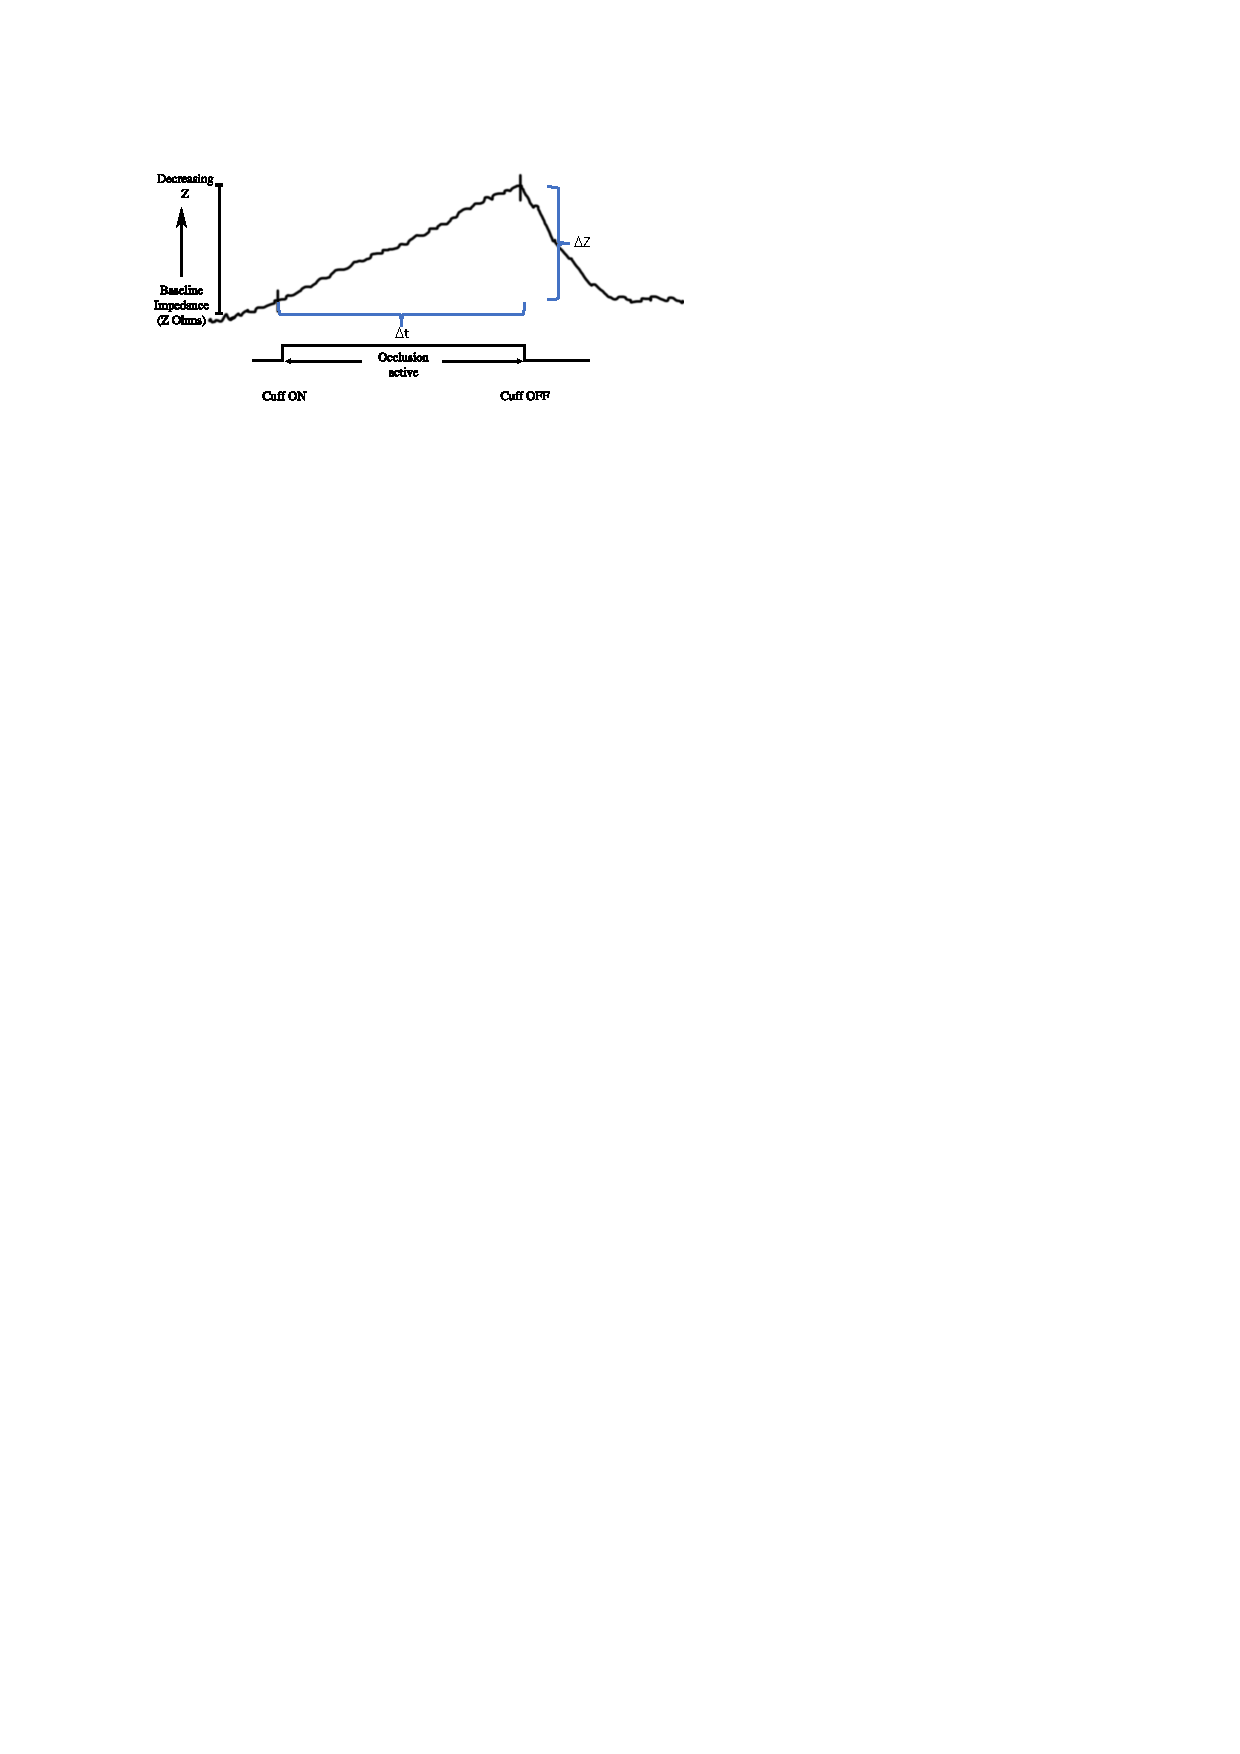
\includegraphics[width=0.85\textwidth,keepaspectratio]{figure_Z_change}
	\caption[Change of baseline impedance during a venous occlusion]{When and occlusion is active in the venous circulation, there is a decrease in impedance as the volume of the limb increases. Adapted from \cite{golden1986assessment}}
	\label{fig:impedance decrease}
\end{figure}

Once the volume and its equivalent in impedanceis known, it is possible to estimate the blood flow. From the Newtonian viewpoint, the flow of a fluid is equal to the change in volume over time. Therefore, blood flow can be derived from the forearm's impedance reading using the equation \ref{eq:DVDT}. Based on that equation, $\rho$ equals the conductivity of the blood, which tends to vary with the individual, although a mean value can be assumed. The cylinder's geometry is limited by the distance of the sensing electrodes ($E_2$ and $E_3$) which denotes the length of $l$. The denominator $R_B$ is equivalent to the basal impedance or the foot of the waveform. From the iPG device, it can be seen that this is the signal that comes from the channel $Z_{DC}$. $\Delta R$ is equivalent to the change of basal impedance ($R_{B2} - R_{B1}$) during a period of time ($t_2 - t_1$).  

\begin{align}
	\label{eq:DVDT}
	\frac{\Delta V}{\Delta t}= \rho \frac{l^2}{R_B^2} \times \frac{\Delta R}{\Delta t}
\end{align} 

In order to make these values more meaningful, they must be converted at a time interval per minutes. In addition, the limb blood flow should be expressed in units of \si{\milli\litre} per \SI{100}{\milli\litre} of limb volume. In this case, the equation can be used as \ref{eq:Q_L}.

\begin{align}
	\label{eq:Q_L}
	\dot{Q_L} = \bigg( \frac{1}{R_B} \bigg) \bigg( \frac{\Delta R}{\Delta t} \bigg) \times 60  \times 100  \tagaddtext{[\si{ml/min.100.ml}]}
\end{align} 

Where $\dot{Q_L}$denotes the blood flow per \SI{100}{\milli\litre} of tissue, $R_B$ represents the impedance base value in \si{\ohm}, $\Delta R_B$ is the change of impedance within ${\Delta t}$ in \si{\sec}.

\subsection{Volume and flow calculation beat by beat}
\label{section procedure flow beat}
Impedance plethysmography also allows for the calculation of the change in volume as well as the blood flow from every heartbeat \cite{costeloe1980continuous, anderson1984impedance, mohapatra1981non, golden1986assessment}. Achieving this calculation is possible if there is high-quality plethysmography waveform. For this reason, the impedance device includes an analogue port known as $Z_{AC}$. As described previously in chapter \ref{chapter design}, this port extracts the plethysmography waveform from the basal impedance channel $Z_{DC}$. As a matter of fact, due to the filtering  as well as amplification stages of the circuit, the signal has been amplified more than \num{2.500} times, thereby providing additional details of the signal's features and increasing its resolution after the digitalisation.

The APA waveform as shown in figure \ref{fig:markers APA} signifies a classic example of a plethysmography wave starting from point $L1$ and finishing in $L2$. Notably, this signal is inverted in impedance because an increase of blood indicates a surge in conductivity. As a result, there is a reduction in impedance of the segment being measured. 

\begin{figure}[!htpb]
	\centering
	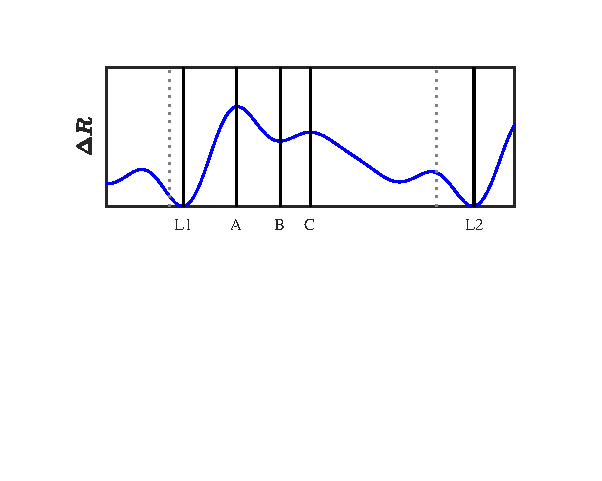
\includegraphics[width=12cm,keepaspectratio]{figure5}
	\caption{Representation of an APA waveform.}
	\label{fig:markers APA}
\end{figure}

The APA signal shows five specific reference points required to calculate volume and blood flow. During the systolic process, two planes are evident in the plethysmography wave. The first one is the upslope of the signal $(L_{1})$ during the isovolumetric contraction of the heart. This point marks the beginning of the plethysmography signal. Next, owing to blood ejection from the heart, the aortic outflow raises the pressure within the circulatory system. Therefore, an increase in blood flow is noticeable, which is pronounced as the maximum amplitude in the plethysmography signal $(A)$. 

During the heart cycle's diastolic development, the next observable reference point in the plethysmography wave is the dicrotic notch. This waveform appears after a decline in pressure within the circulatory system. In the APA wave shown in figure \ref{fig:markers APA}, two points can be seen within this region. The dicrotic notch is located precisely at the landmark $B$ followed by a tiny peak $C$ which marks the post-dicrotic notch segment. 

Finally, the cycle gets completed with the last dip in the APA waveform identified as $L2$. It also marks the beginning of the next volumetric cycle. 

In the wake of these landmarks in the waveform, it is possible to calculate blood flow from the following set of equations adapted from \cite{montgomery2011segmental}. First, the average basal impedance ($R_B$) during the course of a pulse cycle can be calculated by averaging the resistance values at points $L1$ and $L2$. The mathematical operation used in Matlab GUI to calculate this basal impedance between cycles was equation \ref{eq:RB}.

%Note if I want more details check this website http://www.anslab.net/static/helpprofessional/impedancecardiography.html

\begin{align}
	\label{eq:RB}
	R_B = \frac{R_{L1}+R_{L2}}{2} \tagaddtext{[\si{\Omega}]}
\end{align}

Subsequently, the extrapolation of the reference points from the APA pulse given by the Nyboer back-projection \cite{montgomery2011segmental} must be conducted. This value is equivalent to $dR/dt$ in other blood flow equation; instead, two reference points are used. The equation \ref{eq:exht} exhibits the mathematical operation used to calculate this value.

\begin{align}
	\label{eq:exht}
	EXHT = (R_{B}-R_{L1}) + \frac{(t_{B}-t_{L1})(R_{A}-R_{B})}{t_{B}-t_{A}} \tagaddtext{[\si{\Omega}]}
\end{align}

Another key physiological measurement used to calculate blood flow is the heart rate that can be obtained directly from the APA waveform. The HR is equivalent to the difference of time in a cycle multiplied by \SI{60}{\second}. Using equation \ref{eq:hr} the heart rate in beats per minute (\si{bpm}) can be estimated as follows.

\begin{align}
	\label{eq:hr}
	HR = \frac{60}{(t_{L2}-t_{L1})}  \tagaddtext{[\si{bpm}]}
\end{align}

The segmental blood flow beat to beat can be calculated using the Nyboer's equation \ref{eq:DVDT}. Equation \ref{eq:bf} illustrates the equivalent mathematical operation in function of the heart rate that is obtained from equation \ref{eq:hr} as well as the extrapolated APA pulse amplitude denoted by equation \ref{eq:exht}.Due to the fact that the HR has been included in this equation, the units of this formula are \si{\milli\litre\per\min}. 

\begin{align}
	\label{eq:bf}
	BF = HR \times EXHT \times \rho \frac{l^2}{R_B^2} \tagaddtext{[\si{\ml\per\min}]}
\end{align}

where $BF$ represents the blood flow expressed in \si{\milli\litre\per\min}, $\rho$ is the specific resistivity of blood \SI{150}{\ohm\per\cm} \cite{nyober1950electrical, mohapatra1981non}, and $l$ denotes the distance between sensing electrodes ($E2 - E3$).

Blood flow can be observed in different forms. For instance, it can be represented as either flow per total volume of tissue between the potential electrodes or as a fraction of that volume, since clinical use is usually represented as \SI{100}{\milli\litre} of tissue. The equation \ref{eq:bfve} calculates the blood flow per total tissue volume.

\begin{align}
	\label{eq:bfve}
	BFVE = \frac{BF}{V_e} \times \text{1000 ml} \tagaddtext{[\si{\ml\per\min.\litre}]}
\end{align}

where BFVE denotes the blood flow per litre of volume \si{\ml\per\min.\litre}, BF represents the blood flow found in \ref{eq:bf}, $V_e$ is the forearm's segment volume in \si{\cubic\cm} from equation \ref{eq:v_e} and \SI{1000}{\milli\litre} is the scaling factor that converts the volume into litre.

The other option is to denote the rate of blood flow in the standardized form per \SI{100}{\milli\litre} of volume of tissue, also known as Perfusion Index (PI). As a result, the blood flow must be segmented to \SI{100}{\milli\litre} of tissue. The total volume can be derived from equation \ref{eq:v_e}. Thus, the PI can be calculated using the equation  \ref{eq:bfpct}. 

\begin{align}
	\label{eq:bfpct}
	BF_{100ml} = \frac{BF}{V_e} \times \text{100 ml} \tagaddtext{[\si{\bfv}]}
\end{align}

To reiterate, all these flow equations were implemented in Matlab to calculate the blood flow rateduring venous occlusion and beat-to-beat.

\section{Conclusion}
An experiment was set up to measure the changes of impedance that can be converted into blood flow when an occlusion occurs. The entire experiment aims to collect data when three different kinds of occlusion occur: venous occlusion, partial arterial occlusion and total occlusion. The protocol was designed to take \SI{5}{\minute} of resting data followed by \SI{3}{\minute} of readings at the time of each flow restriction.

The data derived from the instruments is in volts \si{\volt} which does not represent a physiological measurement. Therefore, all these equations that were required to convert the data were explained in significant detail. The data sourced from the impedance device was also examined in greater detail in order to better understand and use two methods of measuring blood flow.

In the end, the entire data along with the mathematical operations were input into Matlab where a custom GUI was programmed. From this interface, it is possible to qualify and quantify the data.In addition, filters were applied and a statistical analysis was undertaken. This work adequately complements the design of iPG device, which combines the equations, filters and algorithms presented in this chapter to produce equivalent physiological readings.

%********************************** %Nomenclature found  *************************************
\nomenclature[z-ecg]{ECG}{Electrocardiography}
\nomenclature[z-daq]{DAQ}{Data Acquisition Card}
\nomenclature[z-usb]{USB}{Universal Serial Bus}
\nomenclature[z-vi]{VI}{Virtual Instrument}
\nomenclature[z-gui]{GUI}{Graphic User Interface}
\nomenclature[z-iir]{IIR}{Infinite Impulse Response}
\nomenclature[z-c]{C}{Speed of sound}
\nomenclature[z-ldf]{LDF}{Laser Doppler Flowmetry}
\nomenclature[z-bpu]{BPU}{Blood Perfusion Unit}
\nomenclature[z-pi]{PI}{Perfusion Index}
\nomenclature[z-du]{DU}{Doppler ultrasound}
\nomenclature[z-to]{TO}{Total Occlusion}

